\documentclass[handout]{beamer}
\usepackage{array}
\usepackage{german}
\usepackage{graphicx}
\usepackage[utf8]{inputenc}
\usepackage[T1]{fontenc}
\mode<beamer>{%
\usetheme{Copenhagen}
}
\usepackage[orientation=landscape,size=a3,debug,scale=2.2]{beamerposter}
\title[]{}
\begin{document}
\begin{frame}
\frametitle{%\hspace{0pt plus 1 filll}
MathSem 2025: Felder}
\vspace*{-0.1cm}
\begin{columns}[t,onlytextwidth]
\begin{column}{0.37\textwidth}
\begin{center}
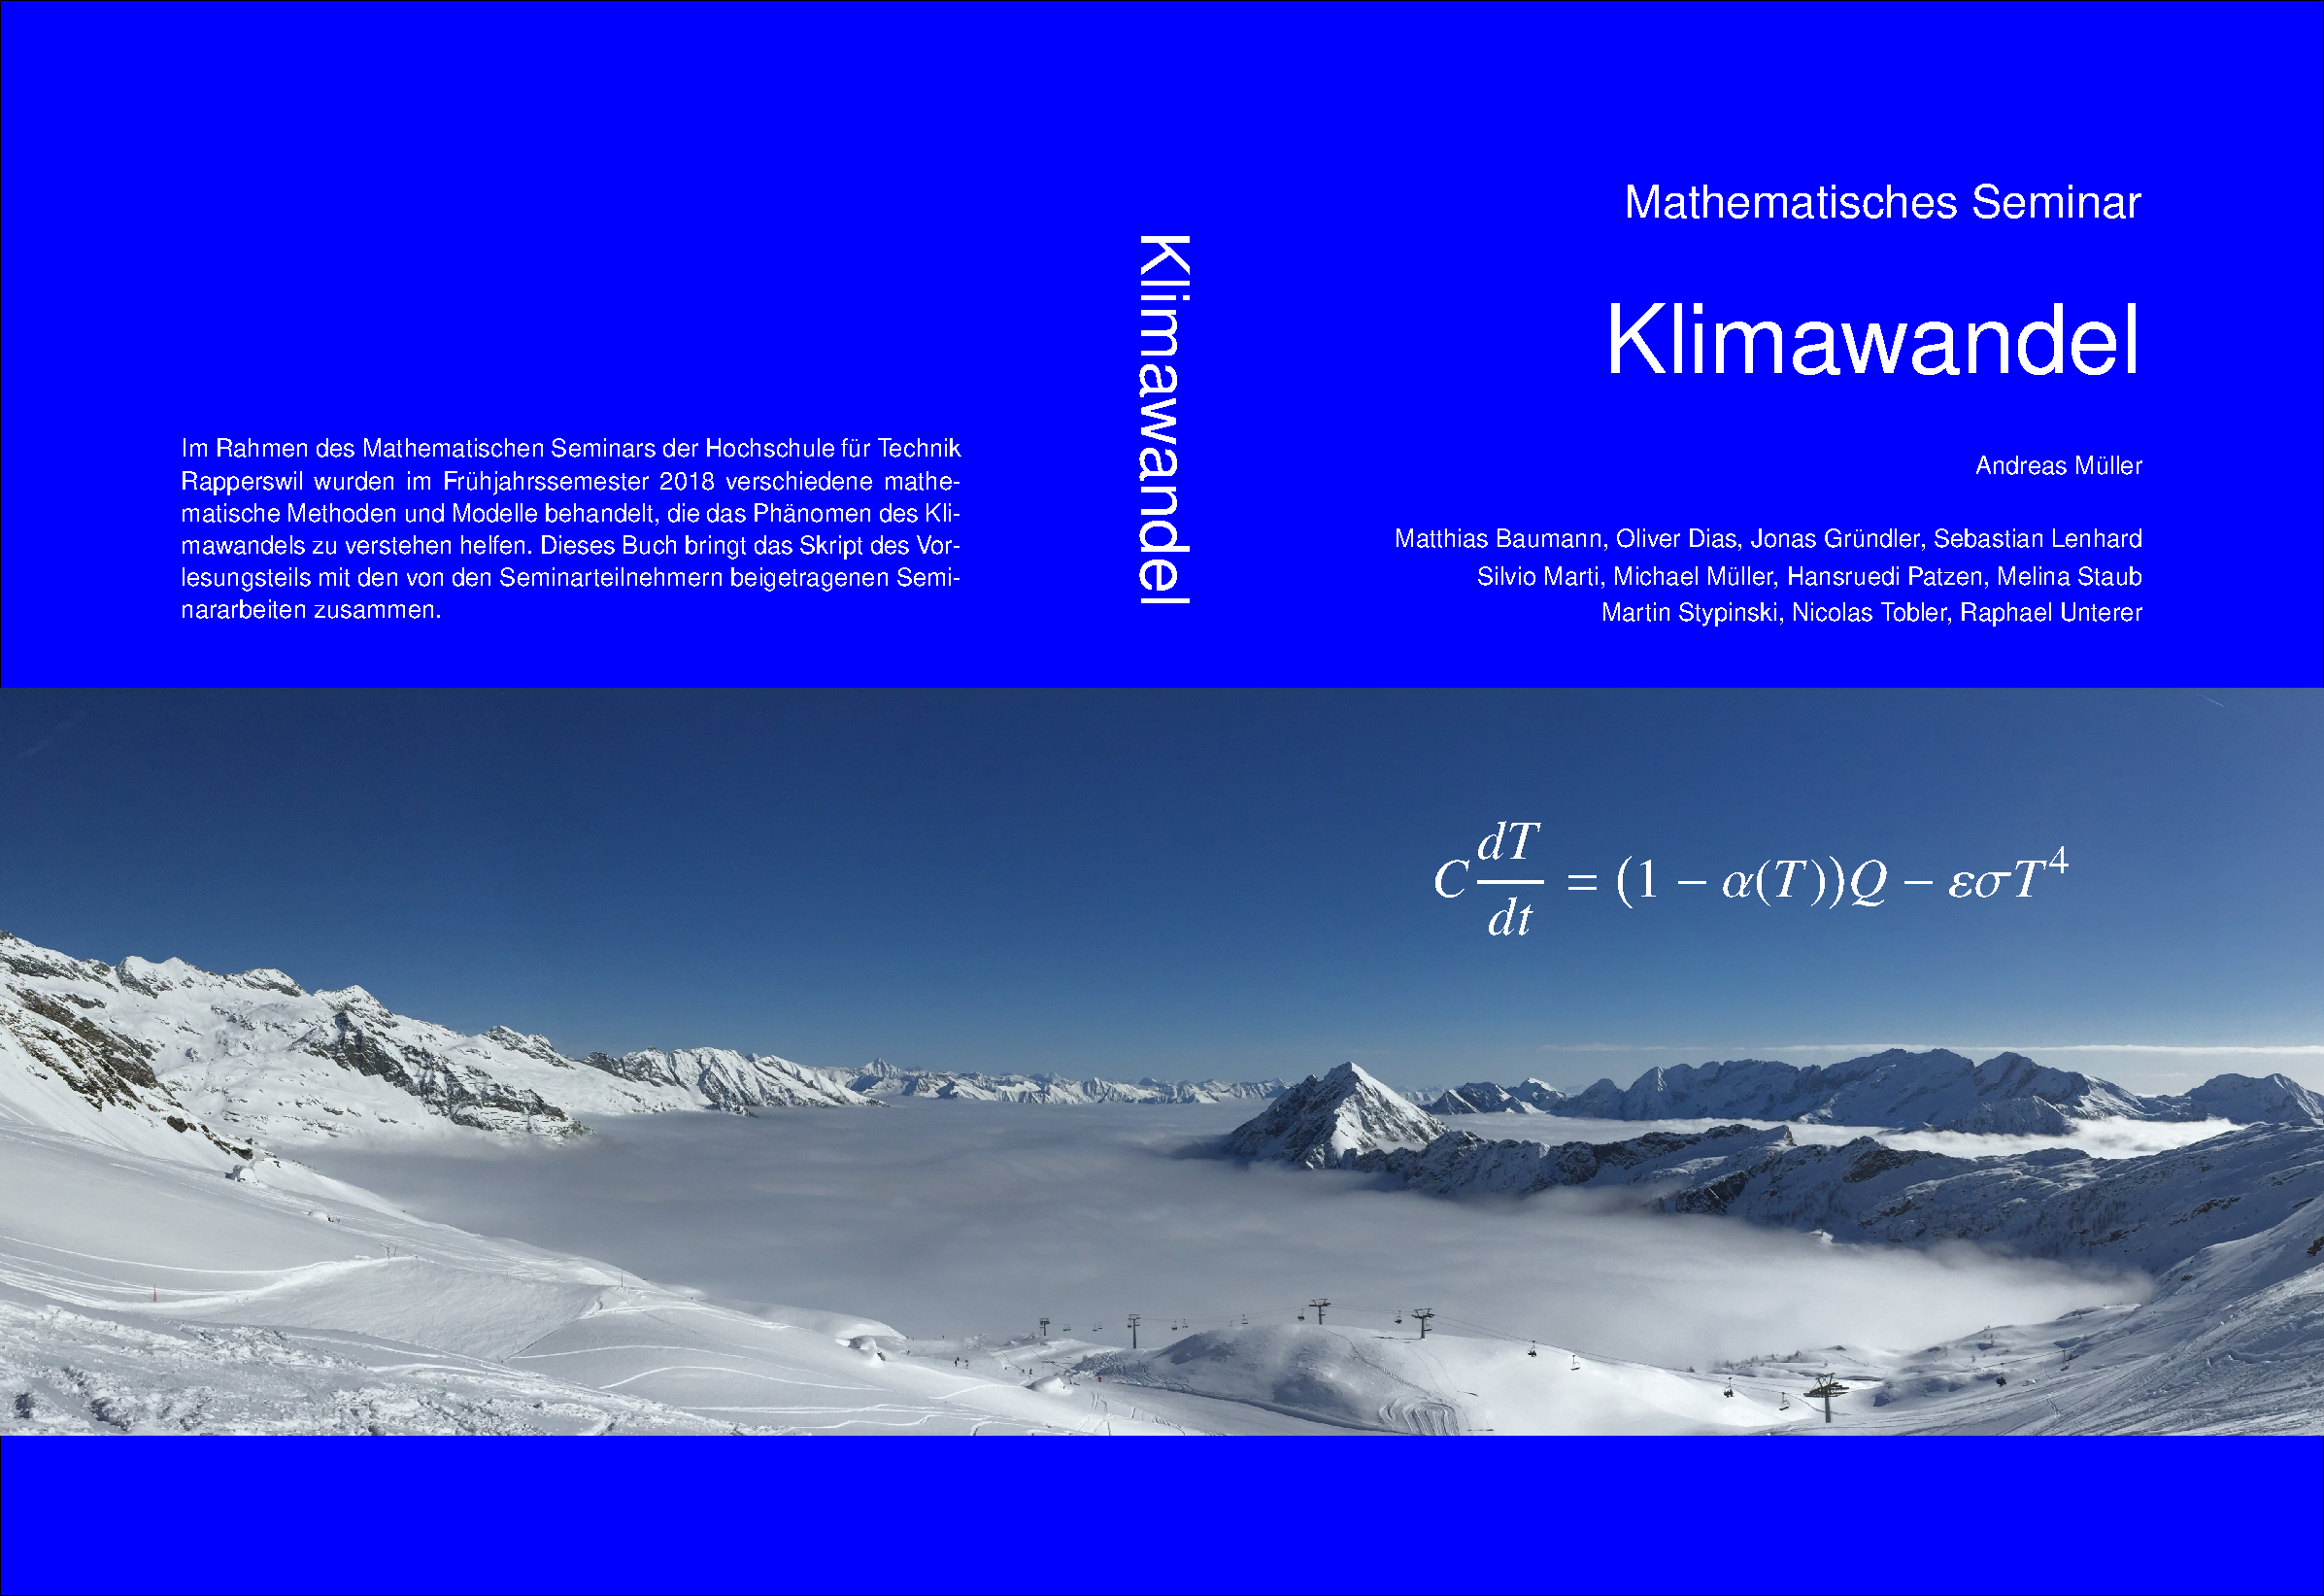
\includegraphics[width=\hsize]{../cover/buchcover.png}
\end{center}
%\vskip 0.2cm
\bigskip
\bigskip
Erscheint~im~Herbst~2025.\\
Anfragen~an~Prof.~Dr.~Andreas Müller,\\
{\texttt{andreas.mueller@ost.ch}}
\bigskip
\bigskip
\bigskip
%\vskip 1.2cm
\end{column}
%
\begin{column}{0.60\textwidth}
\begin{description}
\item[Teil 1:] Grundlagen
\begin{enumerate}
\item Einleitung
\item Eine Fallstudie: Wärme und Temperatur
\item Koordinaten und Tangentialvektoren
\item Differentialformen und Kurvenintegrale
\item 2-Vektoren, 2-Formen und der Satz von Green
\item Der Satz von Gauss
\item $p$-Formen und das Poincaré-Lemma
\item Hodge-Operator, Vektoranalysis und Laplace-Operator
\item Feldgleichungen der klassischen Physik
%\item Numerik der partiellen Differentialgleichungen
\item Zusammenhang und kovariante Ableitung
\item Krümmung
%\item Topologie
\end{enumerate}
\item[Teil 2:] Anwendungen und weiterführende Themen
\begin{enumerate}
\setcounter{enumi}{11}
\item Mike Peng und Pascal Widmer: {\em Maxwell-Gleichungen}
\item Sofia Aaltonen und Ricardo Barbosa: {\em Elastomechanik}
\item Damien Flury: {\em Geometrische Algebra}
%\item Andreas Müller: {\em Differentialoperatoren in orthogonalen Koordinaten}
\setcounter{enumi}{15}
\item Martina Knobel und Gian Kraus: {\em Fourier-Theorie und Feldtheorie}
\item Joël Rechsteiner: {\em Helmholtz-Zerlegung}
\item Alain Keller: {\em Monge-Ampèresche Gleichung}
\item Patrik Müller: {\em Monge-Transport-Theorie}
\item Roman Cvijanovic und Nicola Dall'Acqua: {\em 
Neuronale Netzwerke}
\item Dino Ramcilovic und Tobias Zuber: {\em Nervenfasern}
\item Jero Barahona und Yanick Diggelmann: {\em OpenFOAM Simulation}
\item Flurin Brechbühler und Laurin Heitzer: {\em Turning Waves into Particles}
\item Andrin Kälin und Andrin Rütsche: {\em Gebietsunterteilung und
Parallelisierung}
\item Raphael Unterer: {\em Der Satz von Poincaré-Bendixson}
\item Lukas Schöpf: {\em Reaktions-Diffusions-Gleichungen}
\item Sebastian Eggli und Damian Birchler: {\em Reynolds-Averaging}
\item Michael Schmid: {\em Rossby-Wellen}
\item Robin Eberle: {\em Schallfeld}
\item Emir Arslan und Shaarujan Kamalanathan: {\em Überschallströmung}
\item Nino Briker und Fabian Steiner: {\em Wirbelringe}
\end{enumerate}
\end{description}
\end{column}
\begin{column}{0.01\textwidth}
\llap{\raisebox{-3cm}{\includegraphics{qrcode.pdf}}}
\end{column}
\end{columns}
\end{frame}
\end{document}
